\documentclass[border=5pt]{standalone}
\usepackage{fixltx2e}
\usepackage{tikz}
\usetikzlibrary{shadows}

\usepackage{fontspec}
\setmainfont{Myriad Pro}

\begin{document}

  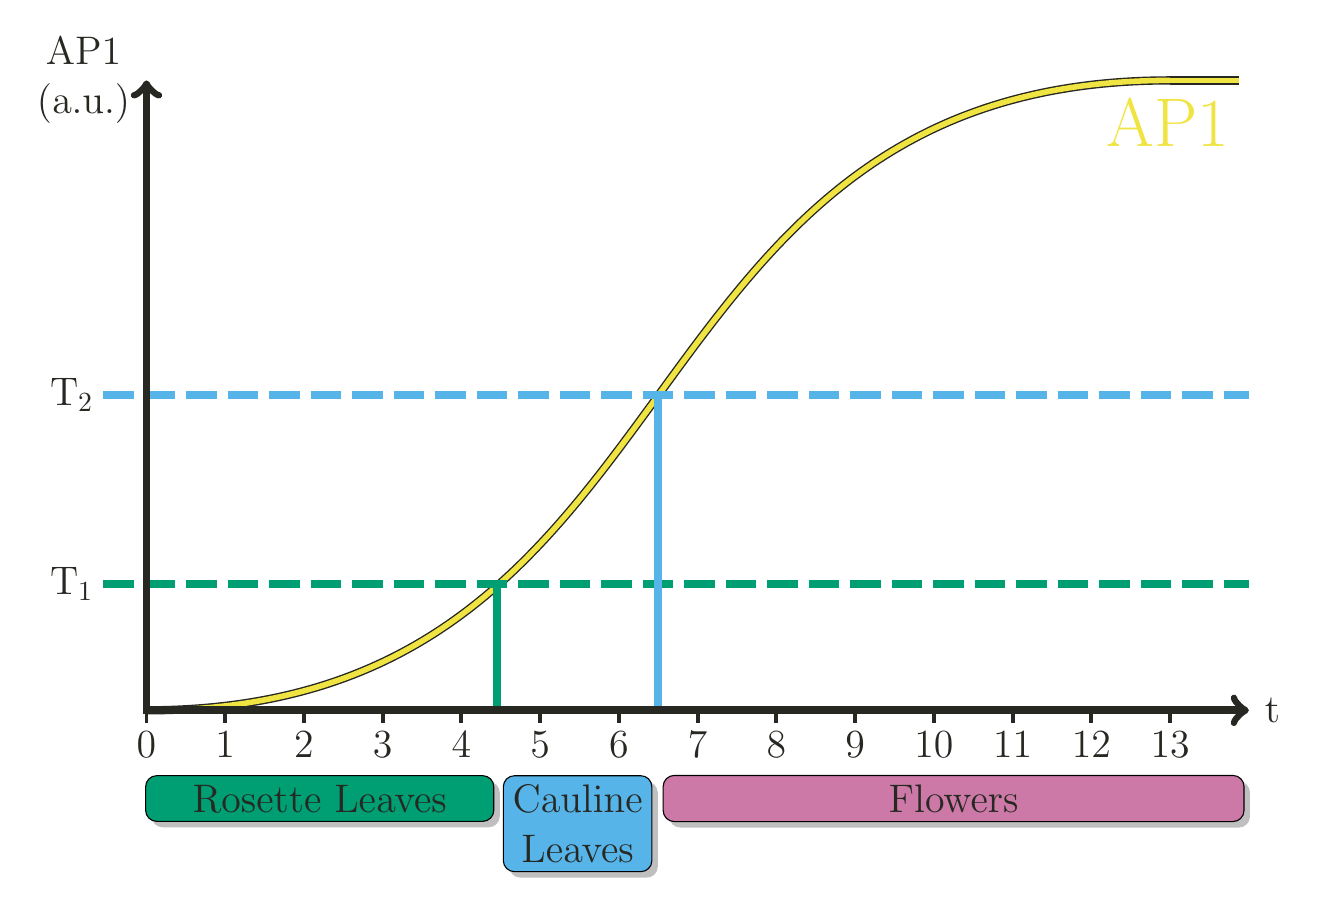
\begin{tikzpicture}[y=8cm]
    % set up colour blind friendly palette
    \definecolor{cbSkyblue}{RGB}{86,180,233}
    \definecolor{cbGreen}{RGB}{0,158,115}
    \definecolor{cbYellow}{RGB}{240,228,66}
    \definecolor{cbPurple}{RGB}{204,121,167}
    \definecolor{monokai}{RGB}{39,40,34}
    \tikzstyle{every node}=[font=\Large, text=monokai]

    %draw AP1 curve
    \coordinate (A) at (13,1);
    \coordinate (B) at (0,0);
    \node[label=225:{\Huge{\textcolor{cbYellow}{AP1}}}] (C) at (14,1) {};
    \draw (B) edge[double=cbYellow,double distance=2pt, line width=0.5pt,draw=monokai, out=360,in=180,looseness = 1.2] (A);    
    \draw (A) edge[double=cbYellow,double distance=2pt, line width=0.5pt,draw=monokai] (C);    

    % label outcomes 
    \node[align=center,fill=cbGreen,draw,rounded corners, drop shadow, inner xsep=17pt] (rose) at (2.2,-0.14) {Rosette Leaves};
    \node[align=center,fill=cbSkyblue,draw,rounded corners, drop shadow] (caul) at (5.475,-0.18) {Cauline\\Leaves};
    \node[fill=cbPurple,draw,rounded corners, drop shadow, inner xsep=81.5pt] (flower) at (10.25,-0.14) {Flowers};
 
    % draw and label thresholds 
    \node[left] (rcThresh) at (-0.55,0.2) {T\textsubscript{1}}; 
    \node[left] (cfThresh) at (-0.55,0.5) {T\textsubscript{2}}; 
    \draw[dash pattern=on 11pt off 4pt, cbGreen, line width=1mm] (rcThresh) -- (14.0,0.2);
    \draw[dash pattern=on 11pt off 4pt, cbSkyblue, line width=1mm] (cfThresh) -- (14.0,0.5);

    % draw lines connecting x-axis to thresholds
    \draw[line width=1mm, color=cbGreen] (4.45,0) -- (4.45,0.2);
    \draw[line width=1mm, color=cbSkyblue] (6.5,0) -- (6.5,0.5);

    % draw and label axes 
    \draw[<->,line width=1mm,color=monokai] (0,1) -- (0,0) -- (14,0);
    \node[align=center] (ylab) at (-0.8,1.0) {AP1\\(a.u.)}; 
    %\node[] (xlab) at (14.3,-0.055) {Time}; 
    \node[] (xlab) at (14.3,-0.0) {t}; 
    % tick marks    
    \foreach \x in {0,1,...,13}{
      \draw[monokai, line width=0.5mm] (\x,0) -- (\x,-0.02);
      \node[monokai] at (\x,-0.055) {\x};
    }

  \end{tikzpicture}

\end{document}
